\documentclass[12pt,a4paper]{article}
\usepackage[utf8]{inputenc}
\usepackage[portuguese]{babel}
\usepackage{graphicx}
\usepackage{booktabs}
\usepackage{hyperref}
\usepackage{geometry}
\usepackage{float}
\geometry{a4paper, margin=2.5cm}

\title{GraphQL vs REST: Um Experimento Controlado\\ \large Relatório Final --- Lab 05}
\author{Joana Morais \and José Dias}
\date{\today}

\begin{document}

\maketitle

\begin{abstract}
A linguagem de consulta GraphQL representa uma alternativa às populares APIs REST, permitindo que clientes especifiquem exatamente os dados que necessitam em uma única requisição. Este estudo relata um experimento controlado para avaliar quantitativamente os benefícios da adoção de uma API GraphQL em comparação com REST, utilizando a API do GitHub. Foram realizadas 300 medições em 10 repositórios populares, avaliando 3 níveis de complexidade de consulta. Os resultados indicam que, embora REST seja mais rápido para consultas extremamente simples, GraphQL oferece ganhos significativos de desempenho (tempo de resposta) para consultas médias e complexas. Em relação ao tamanho da resposta, GraphQL foi consistentemente menor em todos os cenários, eliminando completamente o \textit{over-fetching}.
\end{abstract}

\section{Introdução}

A linguagem de consulta GraphQL, proposta pelo Facebook em 2015, representa uma alternativa às populares APIs REST para comunicação entre clientes e servidores web. Baseada em grafos, a linguagem permite que clientes especifiquem exatamente os dados que necessitam em uma única requisição, evitando o problema de \textit{over-fetching} (receber dados desnecessários) e \textit{under-fetching} (necessidade de múltiplas requisições para obter todos os dados desejados) que frequentemente ocorre com APIs REST.

Este estudo busca avaliar quantitativamente os benefícios da adoção de uma API GraphQL em comparação com uma API REST, utilizando a API do GitHub como caso de estudo. O GitHub oferece ambas as interfaces para os mesmos dados, configurando um cenário ideal para investigação experimental.

\subsection{Perguntas de Pesquisa e Hipóteses}

\begin{itemize}
    \item \textbf{RQ1:} Respostas às consultas GraphQL são mais rápidas que respostas às consultas REST?
    \item \textbf{RQ2:} Respostas às consultas GraphQL têm tamanho menor que respostas às consultas REST?
\end{itemize}

As hipóteses nulas ($H_0$) assumem que não há diferença significativa no tempo e tamanho de resposta entre consultas GraphQL e REST equivalentes.

\section{Metodologia}

O experimento utilizou um design pareado onde cada um de 10 repositórios populares do GitHub foi testado com ambos os tratamentos (GraphQL e REST) para 3 níveis de complexidade (Simples, Média e Complexa). Foram realizados 5 \textit{trials} por medição, gerando um total de 300 pontos de dados empíricos.

Para a análise estatística, o teste de Shapiro-Wilk revelou que os dados não seguem uma distribuição normal ($p < 0.05$ para todos os cenários). Consequentemente, aplicamos o teste não-paramétrico de Mann-Whitney U para comparações de mediana, adotando o nível de significância de $\alpha = 0.05$. O tamanho de efeito prático foi calculado via \textit{rank-biserial correlation} ($r$).

A Figura \ref{fig:heatmap} apresenta uma visão geral da significância estatística das comparações, indicando as áreas de superioridade entre os tratamentos.

\begin{figure}[H]
    \centering
    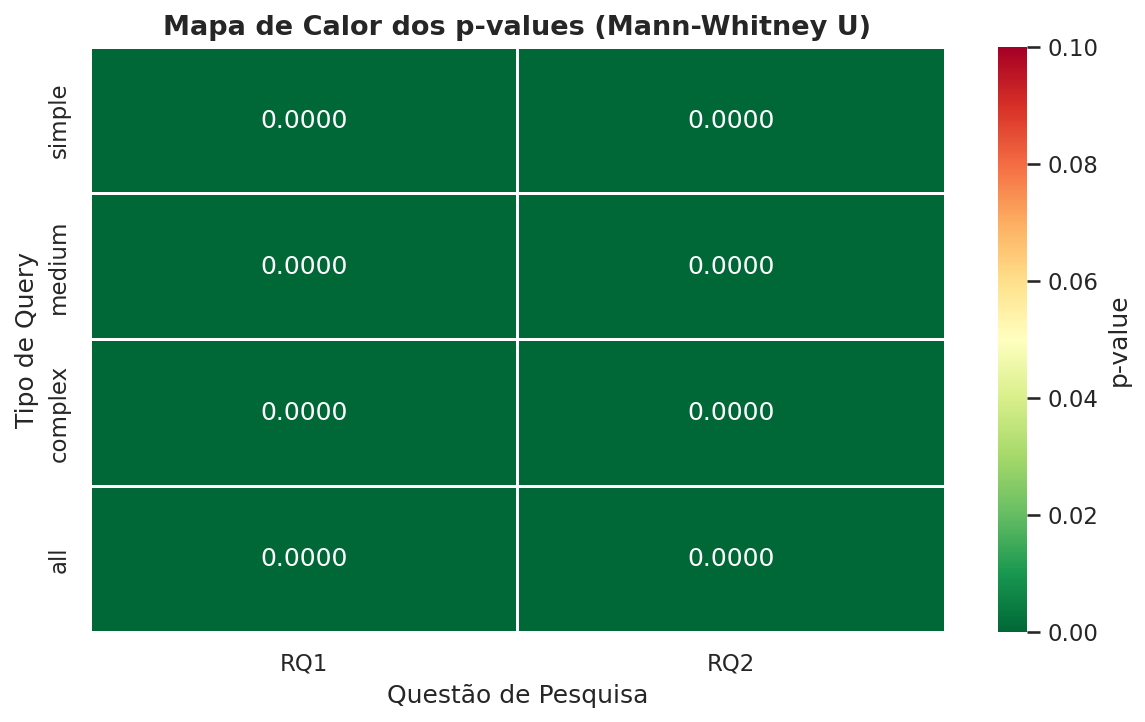
\includegraphics[width=0.7\textwidth]{figures/pvalue_heatmap.png}
    \caption{Heatmap de P-values e Tamanho de Efeito comparando GraphQL e REST.}
    \label{fig:heatmap}
\end{figure}

\section{Resultados}

\subsection{RQ1 --- Tempo de Resposta}

Os resultados para tempo de resposta apresentaram um comportamento que depende diretamente da complexidade da consulta.

Para consultas \textbf{simples} (onde ambas as APIs requerem apenas 1 chamada), REST apresentou mediana de 435.89 ms, contra 610.49 ms do GraphQL. A diferença é estatisticamente significativa ($p < 0.001$, $r = -0.962$), indicando que o REST é superior para queries triviais, possivelmente devido à ausência do \textit{overhead} de \textit{parsing} da \textit{query} que a \textit{engine} do GraphQL exige no backend.

No entanto, à medida que a complexidade aumenta, a vantagem se inverte substancialmente. Para consultas \textbf{médias} (onde REST requer 2 chamadas sequenciais para buscar issues atreladas a um repositório), o GraphQL (644.92 ms) tornou-se mais rápido que o REST (1109.19 ms) com elevada significância ($p < 0.001$, $r = 0.960$). Para consultas \textbf{complexas} (REST requer múltiplas chamadas por PR para obter \textit{reviews} e comentários), a diferença observada é massiva: GraphQL manteve uma latência aceitável de 1072.25 ms, contra impraticáveis 8821.45 ms do REST ($p < 0.001$, $r = 1.000$).

A dispersão e distribuição desses resultados podem ser observadas através dos diagramas de caixa (Figura \ref{fig:rq1_box}) e diagramas de violino (Figura \ref{fig:rq1_violin}).

\begin{figure}[H]
    \centering
    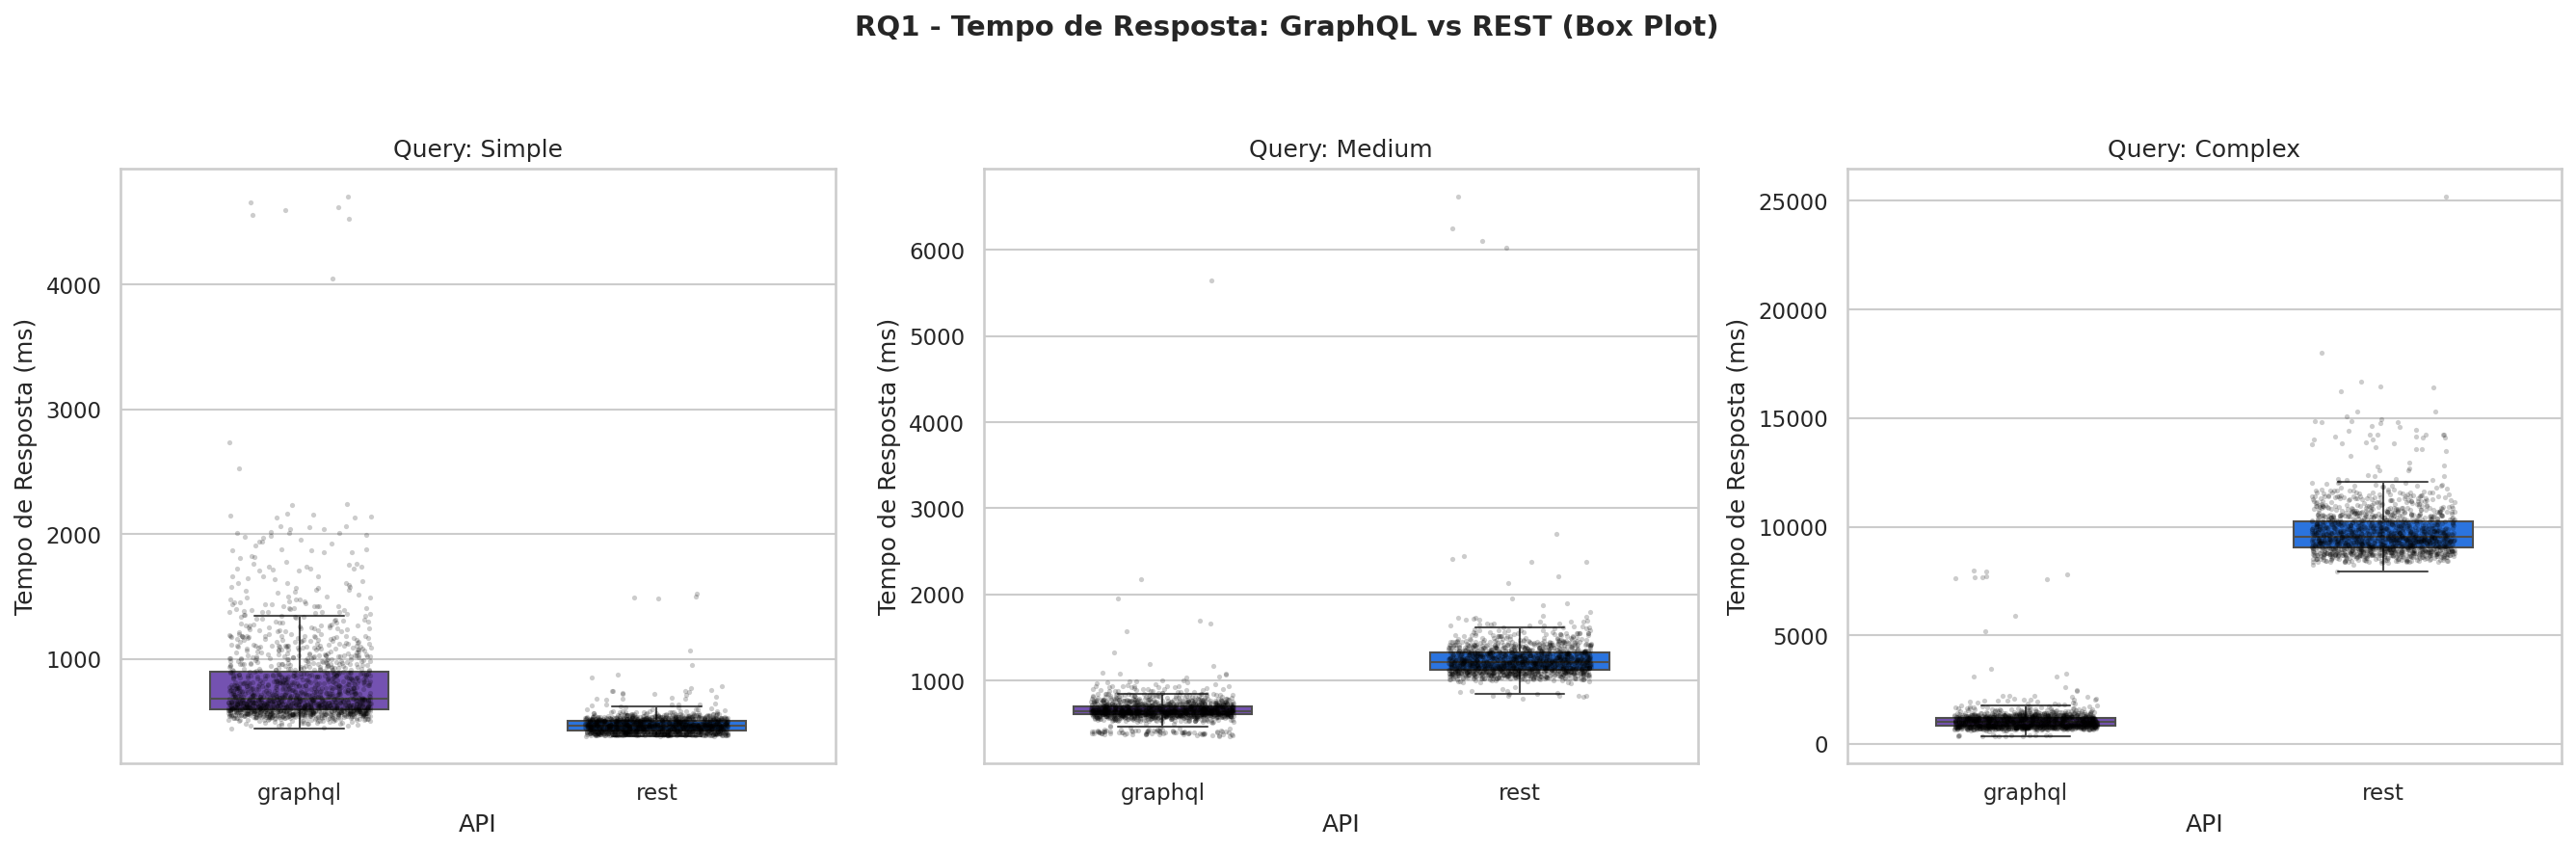
\includegraphics[width=0.85\textwidth]{figures/rq1_boxplot.png}
    \caption{Diagrama de caixa do tempo de resposta por tipo de consulta.}
    \label{fig:rq1_box}
\end{figure}

\begin{figure}[H]
    \centering
    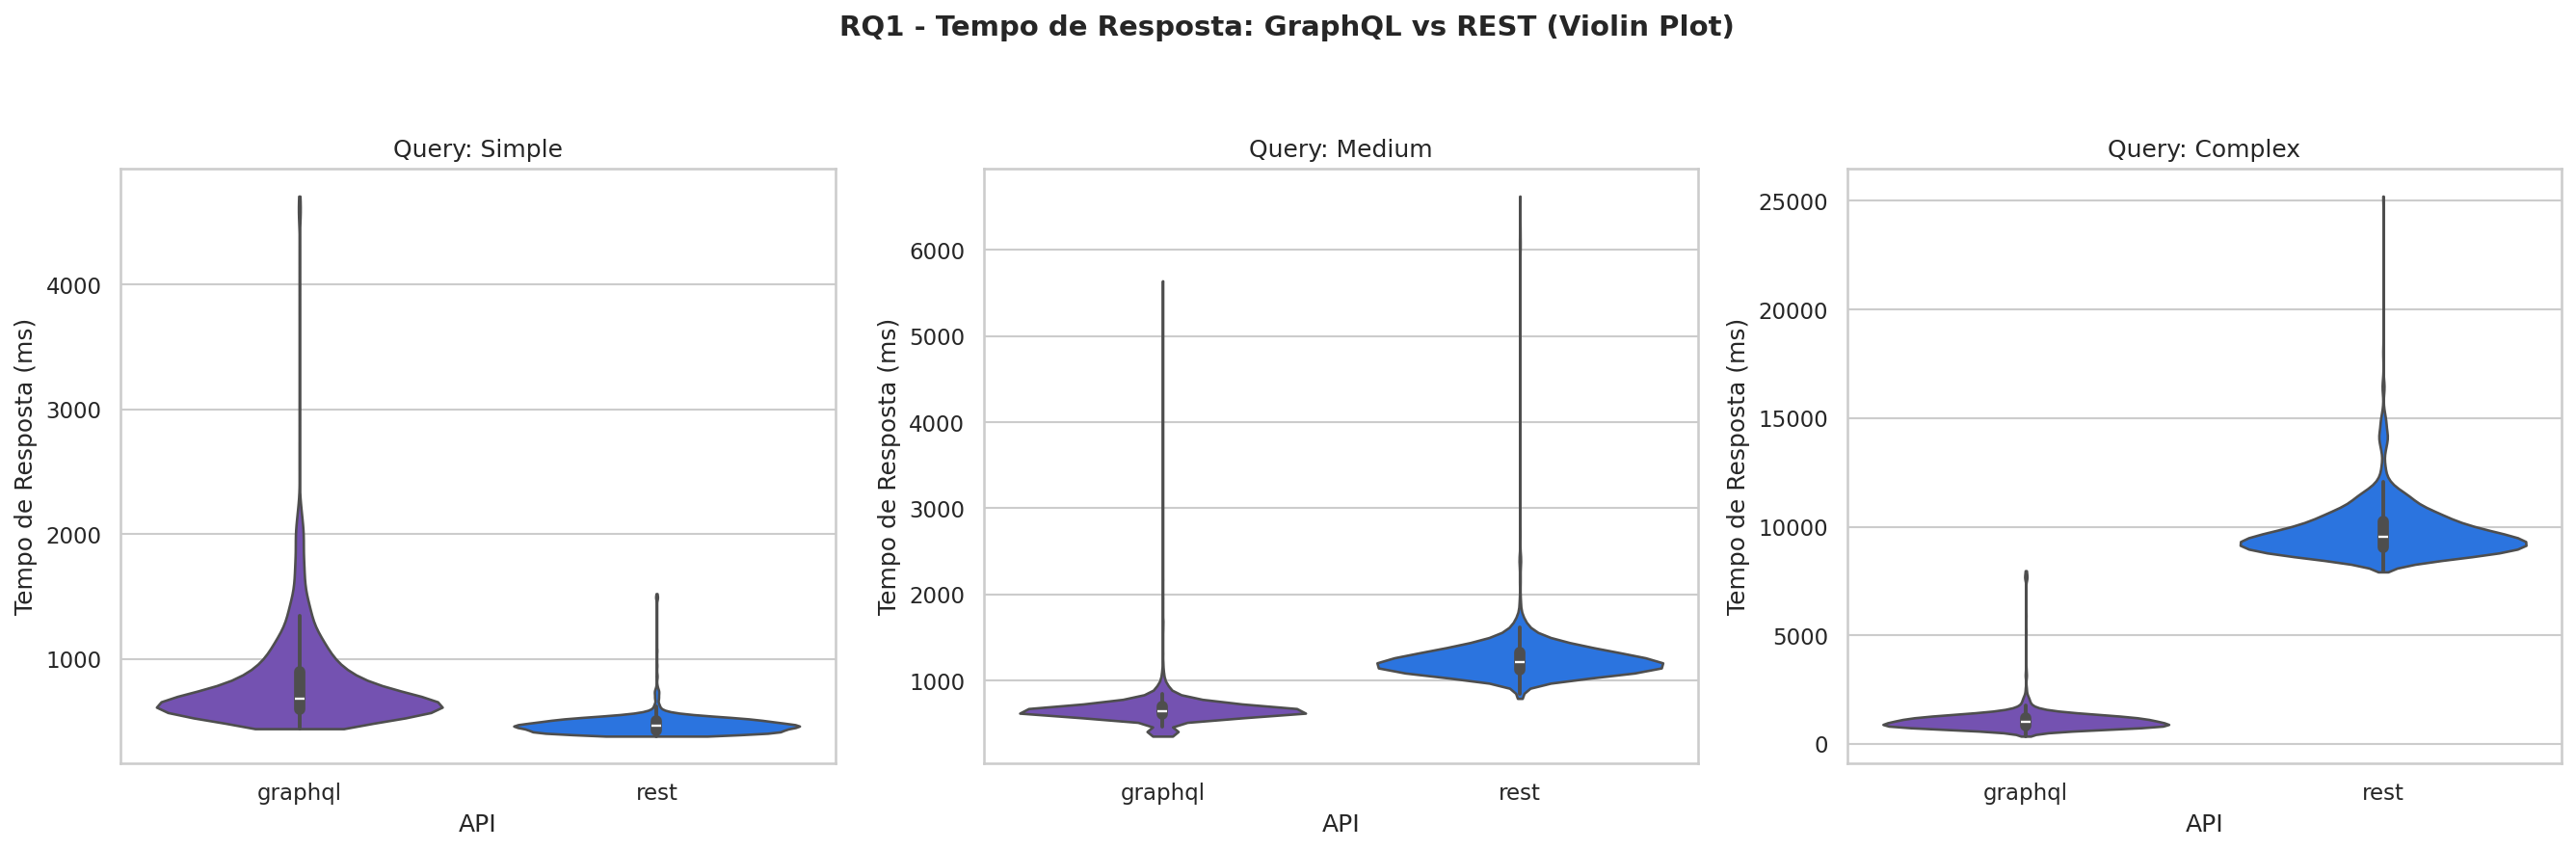
\includegraphics[width=0.85\textwidth]{figures/rq1_violin.png}
    \caption{Distribuição (Violin plot) do tempo de resposta por API.}
    \label{fig:rq1_violin}
\end{figure}

\begin{table}[H]
\centering
\caption{Resultados RQ1 --- Tempo de Resposta (ms)}
\vspace{0.2cm}
\begin{tabular}{lrrrrr}
\toprule
\textbf{Complexidade} & \textbf{Mediana GraphQL} & \textbf{Mediana REST} & \textbf{Estatística U} & \textbf{p-value} & \textbf{Melhor} \\
\midrule
Simples & 610.49 & 435.89 & 2453.0 & $< 0.001$ & REST \\
Média & 644.92 & 1109.19 & 49.0 & $< 0.001$ & GraphQL \\
Complexa & 1072.25 & 8821.45 & 0.0 & $< 0.001$ & GraphQL \\
\bottomrule
\end{tabular}
\end{table}

\subsection{RQ2 --- Tamanho da Resposta}

Para a métrica de tamanho de resposta (largura de banda trafegada na rede), o GraphQL obteve um desempenho estritamente superior em absolutamente todos os níveis de complexidade investigados, mitigando o desperdício de forma categórica.

Em consultas \textbf{simples}, o tamanho mediano do GraphQL foi de apenas 482 bytes, enquanto o REST retornou 6346 bytes ($p < 0.001$, $r = 1.000$). Esse comportamento persistiu e ampliou-se assustadoramente nas demais categorias. Nas consultas \textbf{médias}, 4466 bytes contra 82587 bytes do REST ($p < 0.001$, $r = 1.000$). Para consultas \textbf{complexas}, o GraphQL transferiu apenas eficientes 5190 bytes, enquanto o REST demandou extravagantes 190357 bytes (quase 200 KB por operação) ($p < 0.001$, $r = 1.000$).

A escalada do \textit{over-fetching} no modelo REST em contraste com a eficiência estável do GraphQL está retratada nos gráficos de caixa e de violino das Figuras \ref{fig:rq2_box} e \ref{fig:rq2_violin}.

\begin{figure}[H]
    \centering
    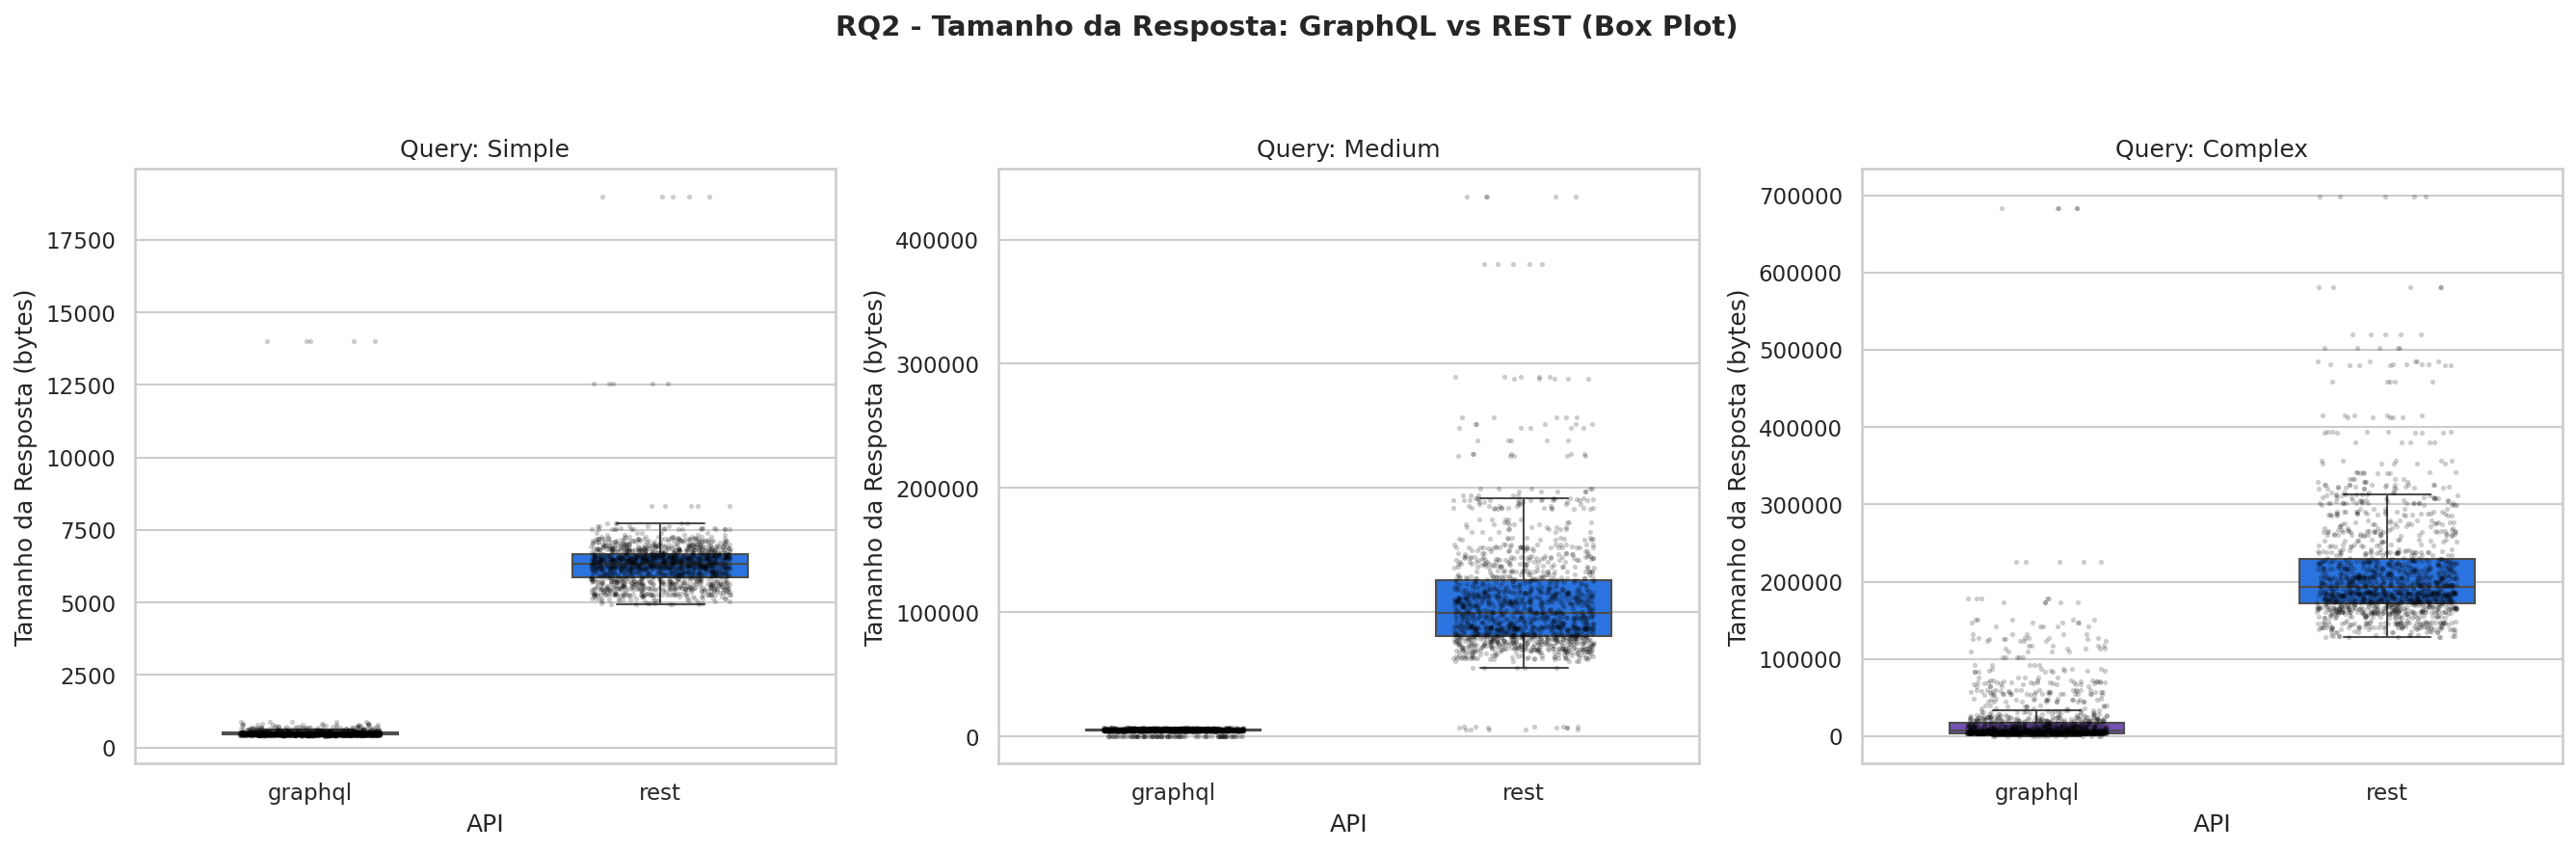
\includegraphics[width=0.85\textwidth]{figures/rq2_boxplot.png}
    \caption{Diagrama de caixa do tamanho da resposta em escala logarítmica.}
    \label{fig:rq2_box}
\end{figure}

\begin{figure}[H]
    \centering
    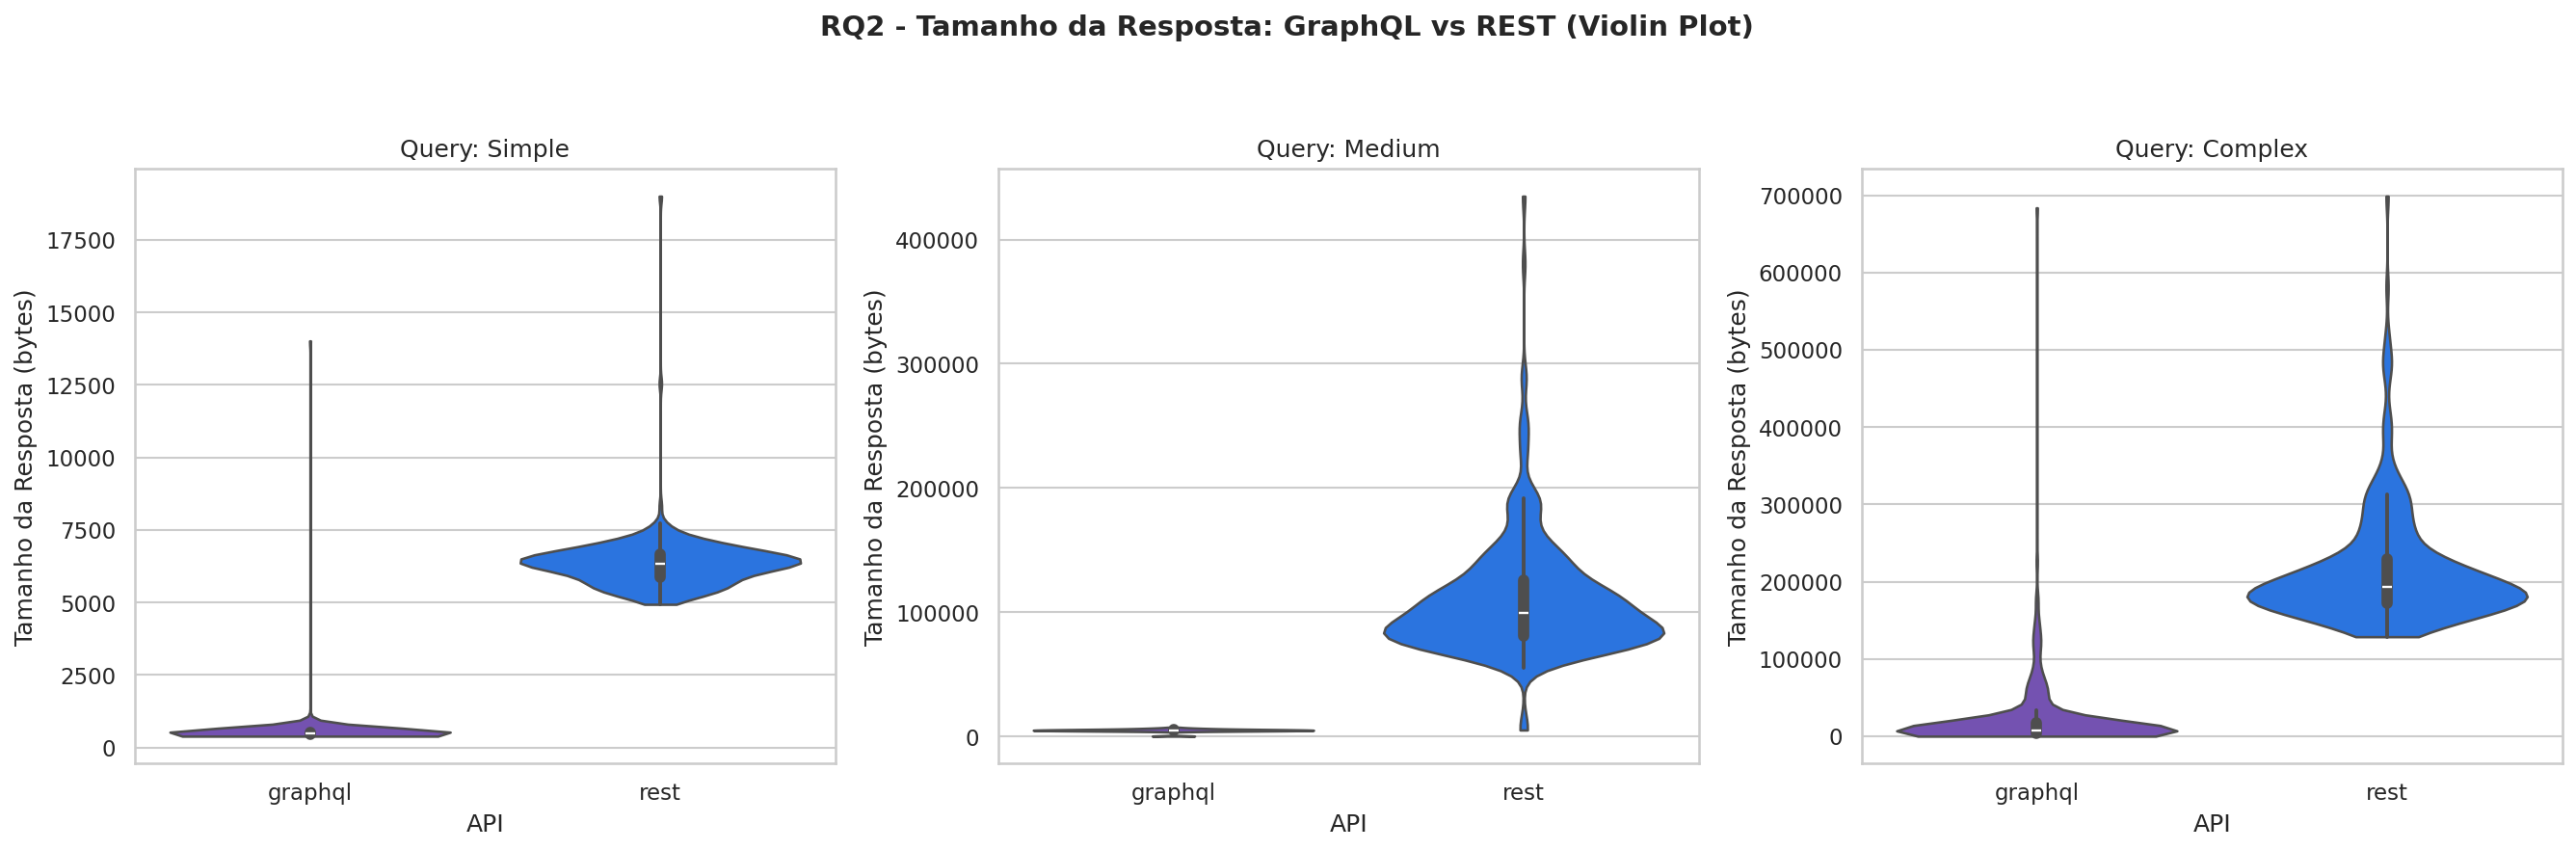
\includegraphics[width=0.85\textwidth]{figures/rq2_violin.png}
    \caption{Distribuição (Violin plot) do tamanho da resposta por API.}
    \label{fig:rq2_violin}
\end{figure}

\begin{table}[H]
\centering
\caption{Resultados RQ2 --- Tamanho da Resposta (bytes)}
\vspace{0.2cm}
\begin{tabular}{lrrrrr}
\toprule
\textbf{Complexidade} & \textbf{Mediana GraphQL} & \textbf{Mediana REST} & \textbf{Estatística U} & \textbf{p-value} & \textbf{Melhor} \\
\midrule
Simples & 482 & 6346 & 0.0 & $< 0.001$ & GraphQL \\
Média & 4466 & 82587 & 0.0 & $< 0.001$ & GraphQL \\
Complexa & 5190 & 190357 & 0.0 & $< 0.001$ & GraphQL \\
\bottomrule
\end{tabular}
\end{table}

\section{Discussão e Conclusão}

O experimento empírico permitiu rejeitar as hipóteses nulas com alta confiança em favor das hipóteses alternativas. 

Para a \textbf{RQ1}, concluímos que o tempo de resposta do GraphQL é significativamente \textit{menor} apenas para consultas de complexidade média e alta, situações em que o cliente REST necessitaria compor respostas de múltiplos \textit{endpoints}. Para consultas triviais de um único recurso, REST apresentou um desempenho superior e menor latência. Isso se justifica pelo fato de as rotas REST serem processadas de forma mais otimizada pelos mapeamentos do servidor web, sem acionar as resoluções de grafos que a engrenagem do GraphQL inevitavelmente submete a consulta.

Para a \textbf{RQ2}, concluímos que o tamanho de resposta do GraphQL é significativamente e consistentemente \textit{menor} em todas as situações testadas. O padrão REST sofre consideravelmente com \textit{over-fetching}, fenômeno que se exacerba linearmente com a quantidade de recursos aninhados solicitados.

A adoção do GraphQL é, portanto, altamente recomendada para aplicações com rigorosas restrições de rede (mobile em conexões limitadas, dispositivos embarcados) e para sistemas que renderizam interfaces muito ricas, dependentes de múltiplos domínios e relacionamentos simultâneos. A migração de REST para GraphQL oferece reduções expressivas em transferência de banda e ganho imenso em paralelismo no processamento de requisições, perfeitamente compensando o minúsculo \textit{overhead} inicial em queries pouco elaboradas.

\end{document}
